\begin{name}
	{\tenchude}{ĐỀ ÔN TẬP SỐ 1}{LỚP TOÁN THẦY PHÁT}{\thoigian}
\end{name}
\setcounter{ex}{0}
\setcounter{bt}{0}
\Opensolutionfile{ans}[ans/ans-Vted-11-2023]

%%==========Câu 1
\begin{ex}%[1D3Y3-3]
	Cấp số cộng $\left(u_{n}\right)$ có $u_{1}=2$ công sai $d=3$ thì $u_{4}$ bằng
	\choice
	{\True $11$}
	{$54$}
	{$14$}
	{$162$}
	\loigiai{
		Ta có $u_{4}=u_{1}+3\cdot d=2+3\cdot 3=11$.
	}
\end{ex}

%%==========Câu 2
\begin{ex}%[2D1Y2-2]
	Cho hàm số $f(x)$ xác định và liên tục trên $\mathbb{R}$ có bảng xét dấu của đạo hàm như sau
	\begin{center}
		
\begin{tikzpicture}
			\tkzTabInit[nocadre=true,lgt=1.2,espcl=1.5,deltacl=0.5]
			{$x$/0.7, $f'(x)$/0.7}
			{$-\infty$,$-1$,$0$,$1$,$2$,$3$,$4$,$+\infty$}
			\tkzTabLine{ ,-,0,+,d,-,0,-,0,+,0,-,0,+, }
		\end{tikzpicture}
	\end{center}
	Số điểm cực trị của hàm số đã cho là
	\choice
	{$3$}
	{$4$}
	{\True $5$}
	{$6$}
	\loigiai{
		Vì hàm số $f(x)$ liên tục trên $\mathbb{R}$ và từ bảng xét dấu đạo hàm $f'(x)$ ta suy ra hàm số $f(x)$ có $5$ điểm cực trị.
	}
\end{ex}

%%==========Câu 3
\begin{ex}%[2D1Y5-4]
	Số điểm chung của hai đường cong $\left(C_{1}\right)\colon y=x^{3}$, $\left(C_{2}\right)\colon y=3x^{2}$ là
	\choice
	{\True $2$}
	{$1$}
	{$3$}
	{$0$}
	\loigiai{
		Xét phương trình $x^3=3x^2 \Leftrightarrow x^{2}(x-3)=0 \Leftrightarrow x=0; x=3$.\\
		Số điểm chung của hai đường cong $\left(C_{1}\right)\colon y=x^{3}$ và $\left(C_{2}\right)\colon y=3x^{2}$ là $2$. 
	}
\end{ex}

%%==========Câu 4
\begin{ex}%[1D2Y2-1]
	Số cách xếp chỗ ngồi cho $3$ học sinh ngồi vào một dãy ghế hàng ngang gồm $5$ ghế, mỗi học sinh ngồi một ghế là?
	\choice
	{$5!$}
	{\True $\mathrm{A}_{5}^{3}$}
	{$\mathrm{C}_{5}^{3}$}
	{$5^{3}$}
	\loigiai{
		Số cách xếp là $\mathrm{A}_{5}^{3}$.
	}
\end{ex}

%%==========Câu 5
\begin{ex}%[2D1Y1-2]
	Cho hàm số $f(x)$ có bảng biến thiên như sau
	\begin{center}
		
\begin{tikzpicture}[>=stealth]
			\tkzTabInit[nocadre=true,lgt=1,espcl=2,deltacl=0.5]{$x$/.7 ,$y'$/.7,$y$/2}
			{$-\infty$ , $-2$ , $2$ , $+\infty$}
			\tkzTabLine{ ,+, $0$ , - , $0$ ,+, }
			\tkzTabVar{-/$-\infty$ ,+/$1$ ,-/$-3$ ,+/$+\infty$}
		\end{tikzpicture}
	\end{center}
	Hàm số đã cho nghịch biến trên khoảng nào dưới đây?
	\choice
	{$(-3; 1)$}
	{\True $(-2; 2)$}
	{$(2;+\infty)$}
	{$(-\infty;-2)$}
	\loigiai{
		Từ bảng biến thiên suy ra hàm số đã cho nghịch biến trên khoảng $(-2; 2)$.
	}
\end{ex}

%%==========Câu 6
\begin{ex}%[2D1Y1-1]
	Tiệm cận đứng của đồ thị hàm số $f(x)=\dfrac{2x-1}{x+1}$
	\choice
	{$y=2$}
	{$x=1$}
	{\True $x=-1$}
	{$y=-1$}
	\loigiai{
		Tập xác định của hàm số $\mathbb{D}=\mathbb{R} \backslash\{-1\}$.\\
		Ta có $\displaystyle \lim_{x \rightarrow-1^{+}}\dfrac{2x-1}{x+1}=+\infty$ suy ra $x=-1$ là tiệm cận đứng của đồ thị hàm số.
	}
\end{ex}

%%==========Câu 7
\begin{ex}%[2D1Y2-2]
	\immini
	{Cho hàm số $f(x)$ có đồ thị như hình vẽ bên. Điểm cực tiểu của hàm số đã cho là
	\choice
	{$x=-1$}
	{$x=0$}
	{\True $x=2$}
	{$x=4$}}
	{\begin{tikzpicture}[line cap=round,line join=round,>=triangle 45,x=1cm,
			y=1cm, scale=0.7]
			% Vẽ 2 trục, điền các số lên trục
			\draw[->] (-2,0)-- (4,0);
			\foreach \x in {2}
			\draw[shift={(\x,0)},color=black] (0pt,2pt)-- (0pt,-2pt) 
			node[below] { $\x$};
			\draw[->,color=black] (0,-1)-- (0,5);
			\foreach \y in {4}
			\draw[shift={(0,\y)},color=black] (2pt,0pt)-- (-1pt,0pt) 
			node[left] {\normalsize $\y$};
			\draw[color=black] (-0.7,0) node[below] {$-1$};
			\draw[color=black] (3.8,.2) node[right] {$x$};
			\draw[color=black] (.1,5) node[right] {\normalsize $y$};
			\draw[color=black] (0pt,-8pt) node[right] {\normalsize $O$};
			\clip(-1.1,-1.1) rectangle (4.06,4.98);
			%Vẽ đồ thị
			\draw[smooth,samples=100,domain=-1.1:4.06] 
			plot(\x,{(\x)^3-3*(\x)^2+4});
			% Vẽ thêm mấy cái râu ria
			\draw (0,0.2)-- (0.2,0.2)-- (0.2,0);
			%Vẽ dấu chấm tròn 
			\fill (0cm,0cm) circle (1.5pt); 
	\end{tikzpicture}}
	\loigiai{
		Hàm số đặt cực tiểu tại điểm $x=2$.
	}
\end{ex}

%%==========Câu 8
\begin{ex}%[2D2B1-3]
	Nghiệm của phương trình $5^{2x-4}=\dfrac{1}{25}$ là
	\choice
	{$x=-4$}
	{$x=-3$}
	{\True $x=1$}
	{$x=3$}
	\loigiai{
		Ta có 
		\allowdisplaybreaks
		$\begin{aligned}[t]
			&\quad 5^{2x-4}=\dfrac{1}{25}\\
			&\Leftrightarrow 5^{2x-4}=5^{-2}\\
			&\Leftrightarrow 2x-4=-2\\
			&\Leftrightarrow x=1.
		\end{aligned}$
	}
\end{ex}

%%==========Câu 9
\begin{ex}%[2D1Y3-4]
	\immini
	{Đường cong ở hình vẽ bên là đồ thị của hàm số nào dưới đây?
	\choice
	{$y=x^3-3x^3$}
	{$y=-x^4+2x^2$}
	{$y=-x^3+3x^2$}
	{\True $y=x^4-2x^2$}}
	{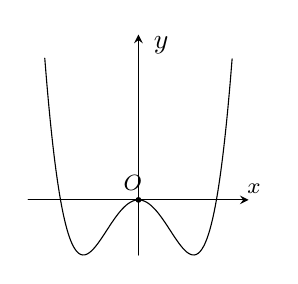
\begin{tikzpicture}[>=stealth,line join=round,line cap=round,font=\footnotesize,scale=0.7]
			% Vẽ 2 trục, điền các số lên trục
			\draw[->] (-2,0)-- (2,0);
			\foreach \x in {}
			\draw[shift={(\x,0)},color=black] (0pt,1pt)-- (0pt,-1pt) 
			node[below] { $\x$};
			\draw[->,color=black] (0,-1)-- (0,3);
			\foreach \y in {}
			\draw[shift={(0,\y)},color=black] (2pt,0pt)-- (-2pt,0pt) 
			node[left] {\normalsize $\y$};
			\draw[color=black] (1.8,.2) node[right] {$x$};
			\draw[color=black] (.1,2.8) node[right] {\normalsize $y$};
			\draw[color=black] (-0.1,0) node[above] {$O$};
			%Vẽ đồ thị
			\draw[smooth,samples=100,domain=-1.7:1.7] 
			plot(\x,{(\x)^4-2*(\x)^2});
			% Vẽ thêm mấy cái râu ria
			%Vẽ dấu chấm tròn 
			\fill (0cm,0cm) circle (1.5pt); 
	\end{tikzpicture}}
	\loigiai{
		Vì đồ thị hàm bậc $4$ có $3$ cực trị và nét cuối cùng đi lên nên đồ thị của hàm số $y=x^4-2x^2$
	}
\end{ex}

%%==========Câu 10
\begin{ex}%[2D1Y1-5]
	Đạo hàm của hàm số $f(x)=x^{\pi}$
	\choice
	{$x^{\pi}\ln{x}$}
	{$\pi x^{\pi}$}
	{\True $\pi x^{\pi-1}$}
	{$\dfrac{x^{\pi+1}}{\pi+1}$}
	\loigiai{
		Ta có $y'=\pi x^{\pi-1}$.
	}
\end{ex}

%%==========Câu 11
\begin{ex}%[2D2B2-6]
	Nghiệm của phương trình $\log_{2}4x=4$ là 
	\choice
	{$x=16$}
	{$x=64$}
	{$x=2$}
	{\True $x=4$}
	\loigiai{
		Điều kiện $4x>0 \Leftrightarrow x>0$.\\
		$\log_2 4x=4 \Leftrightarrow 4x=16 \Leftrightarrow x=4$.
	}
\end{ex}

%%==========Câu 12
\begin{ex}%[2D2B3-7]
	Với $a$ là số thực tùy ý khác $0$. Giá trị của $\log_2 2a^2$ bằng
	\choice
	{$1+2\log_2 a$}
	{$1+\dfrac{1}{2}\log_2 a$}
	{\True $1+2\log_2 \left| a \right |$}
	{$1+\dfrac{1}{2}\left| a \right |$}
	\loigiai{
		$\log_2 2a^2=\log_2 2+\log_2 a^2=1+2\log_2\left| a \right |$.
	}
\end{ex}

%%==========Câu 13
\begin{ex}%[2D2B4-8]
	Với $a$, $b$ là các số thực dương tùy ý khác $1$, khi đó $a^{\log b}$ bằng
	\choice
	{\True $b^{\log a}$}
	{$10^{\log_a b}$}
	{$a^{\log_b 10}$}
	{$10^{\log_b a}$}
	\loigiai{
		Ta có $a^{\log b}=b^{\log a}$.
	}
\end{ex}

%%==========Câu 14
\begin{ex}%[2D3B1-9]
	$\displaystyle \int (3x^2-2x) \mathrm{d}x$ bằng
	\choice
	{\True $x^3-x^2+C$}
	{$3x^3-x^2+C$}
	{$x^3-2x+C$}
	{$6x-2+C$}
	\loigiai{
		Ta có $\displaystyle \int (3x^2-2x) \mathrm{d}x=x^3-x^2+C$.
	}
\end{ex}

%%==========Câu 15
\begin{ex}%[2D3B2-1]
	Nếu $\displaystyle \int_{1}^{2}f(x)\mathrm{d}x=-1$ và $\displaystyle \int_{1}^{3}f(x)=2$ thì $\displaystyle\int_{2}^{3} f(x)\mathrm{d}x$ bằng
	\choice
	{$1$}
	{\True $3$}
	{$-3$}
	{$-1$}
	\loigiai{
		Ta có 
		$\displaystyle\int_{1}^{3}f(x)\mathrm{d}x=\displaystyle\int_{1}^{2}f(x)\mathrm{d}x+\int _{2}^{3}f(x)\mathrm{d}x$\\
		$\Rightarrow 2=-1+\displaystyle\int_{2}^{3}f(x)\mathrm{d}x$\\
		$\Leftrightarrow \displaystyle\int_{2}^{3}f(x)\mathrm{d}x=3$.
	}
\end{ex}

%%==========Câu 16
\begin{ex}%[2D3B3-1]
	$\displaystyle \int 3^x \mathrm{d}x$ bằng
	\choice
	{$3^x\ln{x}+C$}
	{$\dfrac{3^{x+1}}{x+1}+C$}
	{\True $\dfrac{3^x}{\ln{3}}+C$}
	{$x\cdot 3^{x-1}+C$}
	\loigiai{
		Ta có $\displaystyle \int 3^x \mathrm{d}x=\dfrac{3^x}{\ln{3}}+C$.
	}
\end{ex}

%%==========Câu 17
\begin{ex}%[2D3B4-1]
	Nếu $\displaystyle \int_{1}^{2}f(x)\mathrm{d}x=2$ thì $\displaystyle\int_{1}^{2}[f(x)+2x]\mathrm{d}x$
	\choice
	{$1$}
	{\True $5$}
	{$4$}
	{$0$}
	\loigiai{
		Ta có $\displaystyle\int_{1}^{2}[f(x)+2x]\mathrm{d}x=\displaystyle \int_{1}^{2}f(x)\mathrm{d}x+\displaystyle \int_{1}^{2}2x\mathrm{d}x=2+(4-1)=5$.
	}
\end{ex}

%%==========Câu 18
\begin{ex}%[2D4Y1-1]
	Số phức liên hợp của $z=3-4i$ là
	\choice
	{$-3-4i$}
	{\True $3+4i$}
	{$-3+4i$}
	{$3-4i$}
	\loigiai{
		Ta có $z=3-4i$ suy ra $\overline{z}=3+4i$.
	}
\end{ex}

%%==========Câu 19
\begin{ex}%[2D4B1-1]
	Cho $2$ số phức $z_1=5+2i$ và $z_2=1-4i$. Số phức $z_1+3z_2$
	bằng
	\choice
	{\True $8-10i$}
	{$-2+i$}
	{$1-2i$}
	{$-2-i$}
	\loigiai{
		Ta có $z_1+3z_2=5+2i+3(1-4i)=8-10i$.
	}
\end{ex}

%%==========Câu 20
\begin{ex}%[2D4Y2-1]
	Trong mặt phẳng tọa độ $Oxy$, điểm $M(-2;1)$ biểu diễn số phức $z$ khi đó
	\choice
	{$z=2-i$}
	{\True $z=-2+i$}
	{$z=1-2i$}
	{$z=-2-i$}
	\loigiai{
		Điểm $M(-2;1)$ là điểm biểu diễn của số phức $z=-2+i$.
	}
\end{ex}

%%==========Câu 21
\begin{ex}%[2H2Y1-1]%[text hóa đề Vted 2023]%[Huỳnh Xuân Tín]
	Cho khối nón có bán kính đáy bằng $2$, chiều cao bằng $3$. Thể tích của khối nón đã cho bằng
	\choice
	{$12\pi$}
	{$18\pi$}
	{\True $4\pi$}
	{$6\pi$}
	\loigiai{
		Ta có $V=\dfrac{1}{3}\cdot \pi \cdot r^2\cdot h=\dfrac{1}{3}\cdot \pi \cdot 2^2\cdot 3=4\pi$.
	}
\end{ex}	

%%==========Câu 22
\begin{ex}%[2H1B3-2]%[text hóa đề Vted 2023]%[Huỳnh Xuân Tín]
	Một khối chóp tứ giác có đáy là hình vuông cạnh bằng $3$ và chiều cao bằng $10$. Thể tích của khối chóp đó bằng
	\choice
	{\True $30$}
	{$90$}
	{$270$}
	{$15$}
	\loigiai{
		Diện tích đáy của khối chóp đã cho là $3^2=9$, có đường cao của khối chóp là $h=10$.\\
		Thể tích của khối chóp đó là $V=\dfrac{1}{3}\cdot S\cdot h=\dfrac{1}{3}\cdot9\cdot10=30$.		
	}
\end{ex}	

%%==========Câu 23
\begin{ex}%[2H1B3-2]%[text hóa đề Vted 2023]%[Huỳnh Xuân Tín]
	Thể tích của khối hộp chữ nhật $ABCD \cdot A' B' C' D'$ có $A B=3$, $A C=5$, $A A'=8$ bằng
	\choice
	{$120$}
	{$32$}
	{\True $96$}
	{$60$}
	\loigiai{
		\immini
		{Ta có $BC=\sqrt{AC^2-AB^2}=\sqrt{5^2-3^2}=4$.\\
		Khi đó thể tích khối hộp chữ nhật đã cho là
		$V=AA'\cdot AB\cdot BC=8\cdot 3\cdot 4=96$.}
		{\begin{tikzpicture}[scale=1,>=stealth, font=\footnotesize, line join=round, line cap=round]
				\tkzDefPoints{0/0/A,-1.3/-1.1/B,2/-1.1/C}
				\coordinate (D) at ($(A)+(C)-(B)$);
				\coordinate (A') at ($(A)+(0,2.5)$);
				\tkzDefPointsBy[translation=from A to A'](B,C,D){B'}{C'}{D'}
				\tkzDrawPolygon(A',B',B,C,D,D')
				\tkzDrawSegments(B',C' C',D' C,C')
				\tkzDrawSegments[dashed](A,B A,D A,A' A,C)
				\tkzDrawPoints[fill=black](A,B,D,C,A',B',C',D')
				\tkzLabelPoints[above](A',D')
				\tkzLabelPoints[below](A,B,C)
				\tkzLabelPoints[left](B')
				\tkzLabelPoints[right](C',D)
		\end{tikzpicture}}		
	}
\end{ex}	

%%==========Câu 24
\begin{ex}%[2H2Y1-2]%[text hóa đề Vted 2023]%[Huỳnh Xuân Tín]
	Cho hình trụ có bán kính đáy $r=3$ và độ dài đường sinh $\ell=5$. Diện tích xung quanh của hình trụ đã cho bằng
	\choice
	{$15\pi$}
	{\True $30\pi$}
	{$45\pi$}
	{$48\pi$}
	\loigiai{
		Diện tích xung quanh của hình trụ có bán kính đáy $r=3$ và độ dài đường sinh $\ell=5$ là $S_{xq}=2\pi\cdot r\cdot \ell=2\pi\cdot3\cdot5=30\pi$.
	}
\end{ex}	

%%==========Câu 25
\begin{ex}%[2H3Y2-4]%[text hóa đề Vted 2023]%[Huỳnh Xuân Tín]
	Trong KG $Oxyz$, mặt phẳng $(P)\colon x+2y-2z+1=0$ đi qua điểm nào dưới đây?
	\choice
	{\True $M(1;2;3)$}
	{$N(1;2;-2)$}
	{$P(-1;2;-3)$}
	{$Q(2;-2;1)$}
	\loigiai{
		Mặt phẳng $(P)\colon x+2y-2z+1=0$ đi qua điểm $M(1;2;3)$.
	}
\end{ex}	

%%==========Câu 26
\begin{ex}%[2H3Y1-3]%[text hóa đề Vted 2023]%[Huỳnh Xuân Tín]
	Trong KG $Oxyz$, toạ độ tâm mặt cầu $(S)\colon (x-1)^2+(y+2)^2+(z-3)^2=16$ là
	\choice
	{$(1;2;3)$}
	{$(-1;-2;-3)$}
	{$(-1;2;-3)$}
	{\True $(1;-2;3)$}
	\loigiai{
		Toạ độ tâm mặt cầu $(S)\colon (x-1)^2+(y+2)^2+(z-3)^2=16$ là $I(1;-2;3)$.
	}
\end{ex}

%%==========Câu 27
\begin{ex}%[text hóa đề Vted 2023]%[Huỳnh Xuân Tín]%[2H3Y3-1]
	Trong KG $Oxyz$, cho đường thẳng $d\colon\dfrac{x-1}{1}=\dfrac{y+3}{-2}=\dfrac{z+5}{-3}$. Một vectơ chỉ phương của $d$ có tọa độ
	\choice
	{$(1;-3;-5)$}
	{$(1;-2;3)$}
	{$(-1;3;5)$}
	{\True $(-1;2;3)$}
	\loigiai{
		Một vectơ chỉ phương của $d$ có tọa độ là $(-1;2;3)$.
	}
\end{ex}

%%==========Câu 28
\begin{ex}%[Dự án text đề Vted 2023]%[Hiếu Mai]%[2H3Y3-2]
	Trong KG $Oxyz$, đường thẳng đi qua $A(1;2;3)$ và nhận véctơ $\vv{u}=(-1;2;2)$ làm véctơ chỉ phương có PTTS là
	\choice
	{$\heva{
			x&=-1+t
			\\
			y&=2+2t
			\\
			z&=2+3t
		}$}
	{\True $\heva{
			x&=1-t
			\\
			y&=2+2t
			\\
			z&=3+2t
		}$}
	{$\heva{
			x&=1+t
			\\
			y&=2+2t
			\\
			z&=3+2t
		}$}
	{$\heva{
			x&=-1-t
			\\
			y&=2+2t
			\\
			z&=3+3t
		}$}
	\loigiai{
		Đường thẳng đi qua $A(1;2;3)$ và nhận véctơ $\vv{u}=(-1;2;2)$ làm véctơ chỉ phương có PTTS là
		$$\heva{
			x&=1-t
			\\
			y&=2+2t
			\\
			z&=3+2t
		}
		$$
	}
\end{ex}

%%==========Câu 29
\begin{ex}%[Dự án text đề Vted 2023]%[Hiếu Mai]%[1D5G2-7]
	Chọn ngẫu nhiên hai số phân biệt từ $15$ số nguyên dương đầu tiên. Xác suất để tích của hai số được chọn là một số chẵn bằng
	\choice
	{$\dfrac{1}{5}$}
	{$\dfrac{4}{15}$}
	{\True $\dfrac{11}{15}$}
	{$\dfrac{4}{5}$}
	\loigiai{
		Số phần tử của không gian mẫu
		$$
		n(\Omega)=\mathrm{C}_{15}^{2}=105
		$$
		Gọi $ A $ là biến cố: \lq\lq Tích hai số được chọn là một số chẵn\rq\rq. Khi đó, biến cố đối của $ A $ là: \lq\lq Tích hai số được chọn là một số lẻ\rq\rq. Biến cố $ \overline{A} $ chỉ xảy ra khi cả hai số được chọn đều là số lẻ, suy ra
		$$
		n(\overline{A})=\mathrm{C}_{8}^{2}=28
		$$
		Xác suất xảy ra biến cố $ A $:
		$$
		P(A)=1- P(\overline{A})=1-\dfrac{28}{105}=\dfrac{11}{15}
		$$
	}
\end{ex}

%%==========Câu 30
\begin{ex}%[Dự án text đề Vted 2023]%[Hiếu Mai]%[2D1B3-1]
	Giá trị lớn nhất của hàm số $f(x)=-x^3+48x$ trên đoạn $\left[-7;5\right]$ bằng
	\choice
	{$127$}
	{\True $128$}
	{$115$}
	{$7$}
	\loigiai{
		Tập xác định $\mathscr{D}=\mathbb{R}$.\\
		Đạo hàm $f'(x)=-3x^{2}+48$.\\
		Ta có $f'(x)=0 \Leftrightarrow -3x^{2}+48=0 \Leftrightarrow
		\hoac{x&=4\\x&=-4.}$\\
		Xét trên đoạn $\left[-7;5\right]$ thì
		\begin{align*}
			f(-7) &= 7
			\\
			f(-4) &=-128
			\\
			f(4) &= 128
			\\
			f(5) &= 115
		\end{align*}
		Do vậy giá trị lớn nhất của $f(x)$ trên đoạn $\left[-7;5\right]$ là $128$.
	}
\end{ex}

%%==========Câu 31
\begin{ex}%[Dự án text đề Vted 2023]%[Hiếu Mai]%%[2D2B5-2]
	Tập nghiệm của bất phương trình $\log_2 \left(x^2-x\right) \le 1$ là
	\choice
	{\True $\left[-1;0 \right) \cup \left(1;2 \right] $}
	{$\left(-\infty;-1 \right) \cup \left(2;+\infty \right)$}
	{$\left[-1;2 \right]$}
	{$\left(0;1 \right) $}
	\loigiai{
		Giải bất phương trình
		\begin{align*}
			\log_2 \left(x^2-x\right) \le 1
			\Leftrightarrow
			&\heva{
				x^2-x &\le 2^1
				\\ 
				x^2-x&>0
			}
			\\
			\Leftrightarrow
			&\heva{
				&-1 \le x \le 2
				\\ 
				&x < 0 \lor x > 1
			}
			\\
			\Leftrightarrow
			&-1 \le x < 0 \lor 1 < x \le 2
		\end{align*}
		Vậy bất phương tình có tập nghiệm $S=\left[-1;0 \right) \cup \left(1;2 \right]$.		
	}
\end{ex}

%%==========Câu 32
\begin{ex}%[Dự án text đề Vted 2023]%[Hiếu Mai]%%[2D1B1-1]
	Hàm số $y=-\dfrac{1}{3}x^3+2x^2+5x-1$ đồng biến trên khoảng nào dưới đây?
	\choice
	{$\left(-\infty;-1 \right)$}
	{\True $\left(-1;4 \right)$}
	{$\left(-\infty;5 \right)$}
	{$\left(5;+\infty \right)$}
	\loigiai{
		Tập xác định $\mathscr{D}=\mathbb{R}$.\\
		Đạo hàm $y'=-x^2+4x+5$.\\
		Giải phương trình $y'=0 \Leftrightarrow-x^2+4x+5=0 \Leftrightarrow \hoac{x&=-1\\x&=5.}$\\
		Bảng biến thiên 
		\begin{center}
			
\begin{tikzpicture}
				\tkzTabInit[nocadre=false,lgt=1.2,espcl=2.5,deltacl=0.6]
				{$x$ /0.6,$y’$ /0.6}
				{$-\infty$,$-1$,$5$,$+\infty$}
				\tkzTabLine{,-,0,+,0,-,}
				%				\tkzTabVar{-/$-\infty$,+/$2$,-/$-2$,+/$+\infty$}
			\end{tikzpicture}
		\end{center}
		Dựa vào bảng biến thiên, ta thấy hàm số đã cho đồng biến trên khoảng $\left(-1;5 \right)$.
	}
\end{ex}

%%==========Câu 33
\begin{ex}%[2D4B2-1]
	Cho hái số phức $z_1=4+3i$, $z_2=1-i$. Mô đun của số phức $z_1\cdot\overline{z_2}$ bằng
	\choice
	{\True $5\sqrt{2}$}
	{$4\sqrt{2}$}
	{$5$}
	{$3\sqrt{2}$}
	\loigiai{
		Ta có $z_1\overline{z_2}=(4+3i)(1+i)=1+7i$.\\
		Suy ra $|z_1\cdot\overline{z_2}|=\sqrt{1^2+7^2}=5\sqrt{2}$. 
	}
\end{ex}

%%==========Câu 34
\begin{ex}%[2D3B2-1]
	Cho $\displaystyle\int f(x) \mathrm{\,d}x=x^2+x+C_1$; $\displaystyle\int g(x) \mathrm{\,d}x=x^4+x^3+C_2$. Khi đó $\displaystyle\int\limits_0^1 f(x)\cdot g(x) \mathrm{\,d}x$ bằng
	\choice
	{\True $\dfrac{51}{10}$}
	{$\dfrac{71}{105}$}
	{$4$}
	{$\dfrac{77}{60}$}
	\loigiai{
		Ta có $\displaystyle\int f(x) \mathrm{\,d}x=x^2+x+C_1 \Rightarrow f(x)=2x+1$.\\
		$\displaystyle\int g(x) \mathrm{\,d}x=x^4+x^3+C_2 \Rightarrow g(x)=4x^3+3x^2$.\\
		Vậy $\displaystyle\int\limits_0^1 f(x)\cdot g(x) \mathrm{\,d}x=\displaystyle\int\limits_0^1 (2x+1)(4x^3+3x^2) \mathrm{\,d}x=\displaystyle\int\limits_0^1 (8x^4+10x^3+3x^2) \mathrm{\,d}x=\left(\dfrac{8}{5} x^4+\dfrac{5}{2}x^4+x^3\right) \bigg|_0^1=\dfrac{51}{10}$.
	}
\end{ex}

%%==========Câu 35
\begin{ex}%[1H3B3-3]
	Cho hình hộp chữ nhật $ABCD.A'B'C'D'$ có $AB=2\sqrt{3}a$, $AD=a$, $AA'=\sqrt{3}a$. Góc giữa đường thẳng $A'C$ và mặt phẳng $(ADD'A')$ bằng
	\choice
	{$45^\circ$}
	{$90^\circ$}
	{\True $60^\circ$}
	{$30^\circ$}
	\loigiai{
		\immini
		{Do $ABCD.A'B'C'D'$ là hình hộp chữ nhật nên suy ra $CD \perp (ADD'A')$.\\
		Suy ra góc giữa đường thẳng $A'C$ và mặt phẳng $(ADD'A')$ là góc $\widehat {CA'D}$.\\
		Ta có $A'D=\sqrt{AA'^2+AD^2}=\sqrt{3a^2+a^2}=2a$.\\
		$\tan \widehat{CA'D}=\dfrac{CD}{A'D}=\dfrac{2\sqrt{3}a}{2a}=\sqrt{3} \Rightarrow \widehat{CA'D}=60^\circ$.\\
		Vậy giữa đường thẳng $A'C$ và mặt phẳng $(ADD'A')$ bằng $60^\circ$.}
		{\begin{tikzpicture}[>=stealth,line join=round,line cap=round,font=\footnotesize,scale=0.7]
			\def \a{-1.5} \def \b{-1}\def \c{3.5} \def \h{4}
			\path (.5,.5)coordinate(A) 
			+(\a,\b)coordinate(B)
			+(\c,0)coordinate(D)
			($(B)+(D)-(A)$)coordinate(C)
			+(0,\h)coordinate(C')
			($(B)+(C')-(C)$)coordinate(B')
			($(A)+(C')-(C)$)coordinate(A')
			($(D)+(C')-(C)$)coordinate(D');
			\draw [dashed] (D)--(A')--(A)--(B)(D)--(A)--(C)--(A');
			\draw(B')--(B)--(C)(B')--(C')--(C)--(D)--(D')--(A')--(B')(C')--(D');	
			\foreach \d/\g in {A/160,B/180,C/-90,D/0,A'/90,B'/180,C'/-30,D'/0}
			\fill[black](\d) circle (1pt)+(\g:.35)node{$\d$};
		\end{tikzpicture}}
	}
\end{ex}

%%==========Câu 36
\begin{ex}%[1H3B5-3]
	Cho lăng trụ $ABC.A'B'C'$ có đáy là tam giác vuông tại $A$, $AB=a$, $AC=\sqrt{3}a$ và $AA'=AB'=AC'=2a$. Khoảng cách từ $A$ đến mặt phẳng $(A'B'C')$ bằng
	\choice
	{\True $\sqrt{3}a$}
	{$a$}
	{$2a$}
	{$\sqrt{2}a$}
	\loigiai{
		\immini
		{Gọi $H$ là hình chiếu của $A$ trên mặt phẳng $(A'B'C')$.\\
		Ta có $AA'=AB'=AC'=2a$ suy ra $H$ là tâm đường tròn ngoại tiếp tam giác $A'B'C'$.\\
		Mà $\triangle ABC$ vuông tại $A$ suy ra $\triangle A'B'C'$ vuông tại $A'$ suy ra $H$ là trung điểm của $B'C'$.\\
		Ta có $BC=\sqrt{AB^2+AC^2}=\sqrt{a^2+3a^2}=2a \Rightarrow B'C'=2a \Rightarrow B'H=a$.\\
		Ta có $AH=\sqrt{AB'^2-B'H^2}=\sqrt{4a^2-a^2}=\sqrt{3}a$.\\
		Vậy $\mathrm{d}(A,(A'B'C'))=a\sqrt{3}$.}
		{\begin{tikzpicture}[scale=0.8, font=\footnotesize, line join=round, line cap=round, >=stealth]
			\def\ac{5}
			\def\ab{2.75}
			\def\h{4}
			\def\gocB'{45}
			\path 
			(0,0) coordinate (B')
			(\ac,0) coordinate (C')
			(-\gocB':\ab) coordinate (A')
			($(B')!1/2!(C')$) coordinate (H)
			($(H)+(0,\h)$) coordinate (A)
			($(B')-(A')+(A)$) coordinate (B)
			($(C')-(A')+(A)$) coordinate (C);
			\draw (A')--(A)--(B)--(C)--(C')--(A')--(B')--(A)(B)--(B')(A)--(C) ;
			\draw[dashed] (A')--(C')--(A)--(H)(B')--(C');
			\foreach \x/\g in {A/180,B/-180,C/0,H/-90,A'/-90,B'/-180,C'/0} \fill[black] (\x) circle (1.2pt) node[shift={(\g:7pt)},scale=.8]{$\x$};
		\end{tikzpicture}}
	}
\end{ex}

%%==========Câu 37
\begin{ex}%[2H3B1-3]
	Trong KG $Oxyz$, cho hai điểm $A\left(1;1;1\right), B\left(3;-1;1\right)$. Mặt cầu đường kính $AB$ có phương trình là
	\choice
	{$\left(x-2\right)^2+y^2+\left(z-1\right)^2=4$}
	{\True $\left(x-2\right)^2+y^2+\left(z-1\right)^2=2$}
	{$\left(x+2\right)^2+y^2+\left(z+1\right)^2=2$}
	{$\left(x+2\right)^2+y^2+\left(z+1\right)^2=4$}
	\loigiai{
		Gọi $\left(S\right)$ là mặt cầu nhận $AB$ làm đường kính.\\
		Ta có
		\begin{itemize}
			\item Tâm $I$ là trung điểm $AB\Rightarrow I\left(2;0;1\right)$.
			\item Bán kính $R=\dfrac{1}{2}AB=\sqrt{2}$.
		\end{itemize}
		Khi đó mặt cầu $\left(S\right)$ có phương trình là $\left(x-2\right)^2+y^2+\left(z-1\right)^2=2$.
	}
\end{ex}

%%==========Câu 38
\begin{ex}%[2H3B2-3]
	Trong KG $Oxyz$, cho ba điểm $A\left(1;1;1\right),B\left(0;2;1\right),C\left(1;-1;2\right)$. Mặt phẳng đi qua $A$ vuông góc với $BC$ có phương trình là
	\choice
	{$x+y+z-3=0$}
	{$x-3y+z-1=0$}
	{\True $x-3y+z+1=0$}
	{$x+y+z+3=0$}
	\loigiai{
		Gọi $\left(P\right)$ là mặt phẳng cần tìm.\\
		Ta có $\left(P\right)\perp BC\Rightarrow \vec{BC}=\left(1;-3;1\right)$ là vec-tơ pháp tuyến của $\left(P\right)$.\\
		Khi đó mặt phẳng $\left(P\right)$ đi qua điểm $A$, nhận $\vec{BC}$ làm vec-tơ pháp tuyến nên có phương trình là $x-3y+z+1=0$.
	}
\end{ex}

%%==========Câu 39
\begin{ex}%[2D4K2-3]
	Có bao nhiêu số phức $z$ thỏa mãn điều kiện $z^2=\left|z\right|^2+2\bar{z}$?
	\choice
	{$4$}
	{$2$}
	{\True $3$}
	{$1$}
	\loigiai{
		Gọi $z=x+yi\Rightarrow \bar{z}=x-yi$, với $x,y\in \mathbb{R}$.\\
		Ta có $z^2=\left|z\right|^2+2\bar{z}\\
		\Leftrightarrow \left(x+yi\right)^2=x^2+y^2+2\left(x-yi\right)\\
		\Leftrightarrow x^2-y^2+2xyi=x^2+y^2+2x-2yi\\
		\Leftrightarrow \heva{&x^2-y^2=x^2+y^2+2x\\&2xy=-2y}\Leftrightarrow \heva{&2y^2+2x=0\\&2y\left(x+1\right)=0}\Leftrightarrow \heva{&y^2+x=0\quad (*)\\&\hoac{&y=0\\&x=-1}}$
		\begin{itemize}
			\item Với $y=0$ thế vào (*) ta được $x=0$.
			\item Với $x=-1$ thế vào (*) ta được $y=\pm 1$.
		\end{itemize}
		Vậy có $3$ có phức $z$ thỏa mãn yêu cầu bài toán.
	}
\end{ex}

%%==========Câu 40
\begin{ex}%[2D1K3-1]
	Cho hàm số $f\left(x\right)$ liên tục trên đoạn $\left[-4;4\right]$ và có bảng biến thiên
	\begin{center}
		\begin{tikzpicture}[font=\normalsize,t style/.style={style=solid}]
			\tkzTabInit[nocadre=true,lgt=1.2,espcl=2.5,deltacl=0.5]
			{$x$ /0.75, $y'$/0.75, $y$/1.75}
			{$-4 $,$-3 $,$-1 $,$ 0 $,$ 2 $,$ 4 $}
			\tkzTabLine{  ,+,0 ,-, 0 ,+,0 ,-, 0 ,+,  }
			\path ($(N12)!0.9!(N13)$) node (A1){$-4$}
			($(N22)!0.2!(N23)$) node (A2){$4$}
			($(N32)!0.9!(N33)$) node (A3){$2$}
			($(N42)!0.2!(N43)$) node (A4){$3$}
			($(N52)!0.9!(N53)$) node (A5){$-3 $}
			($(N62)!0.2!(N63)$) node (A6){$1$};
			\foreach \x/\y in {A1/A2,A2/A3,A3/A4,A4/A5,A5/A6}{
			\draw[-stealth] (\x)--(\y);
			}
		\end{tikzpicture}
	\end{center}
	Có bao nhiêu số thực $m\in \left[-4;4\right]$ để giá trị lớn nhất của hàm số $g\left(x\right)=f\left(x^3-3x+2\right)+f\left(m\right)$ trên đoạn $\left[-1;1\right]$ bằng $1$
	\choice
	{$2$}
	{\True $3$}
	{$4$}
	{$5$}
	\loigiai{
		Đặt $t=x^3-3x+2$ thì $t'=3x^2-3\ge 0, \forall x\in \left[-1;1\right]\Rightarrow \heva{&\underset{[-1;1]}{\mathop{\min }}t=t(1)=0\\&\underset{[-1;1]}{\mathop{\max }}t=t(-1)=4}\Rightarrow t\in \left[0;4\right],\forall x\in \left[-1;1\right]$.\\
		Bài toán trở thành tìm $m\in \left[-4;4\right]$ để $\underset{[0;4]}{\mathop{\max }}\left\{f(t)+f(m)\right\}=1\Leftrightarrow 3+f(m)=1\Leftrightarrow f(m)=-2$.\quad $(*)$
		\begin{center}
			\begin{tikzpicture}[font=\normalsize,t style/.style={style=solid}]
				\tkzTabInit[nocadre=true,lgt=1.2,espcl=2.5,deltacl=0.5]
				{$x$ /0.75, $y'$/0.75, $y$/2.5}
				{$-4 $,$-3 $,$-1 $,$ 0 $,$ 2 $,$ 4 $}
				\tkzTabLine{  , + , 0 , - , 0 , + ,0 , - , 0 , + ,  }
				\path ($(N12)!0.9!(N13)$) node (A1){$-4$}
				($(N22)!0.18!(N23)$) node (A2){$4$}
				($(N32)!0.38!(N33)$) node (A3){$2$}
				($(N42)!0.22!(N43)$) node (A4){$3$}
				($(N52)!0.85!(N53)$) node (A5){$-3 $}
				($(N62)!0.45!(N63)$) node (A6){$1$}
				($(T12)!0.6!(T13)$)coordinate(M)
				($(T22)!0.6!(T23)$)coordinate(N);
				\draw[blue,thick] (M)--(N)node[pos=0.5,sloped,below]{$f(m)=-2$};
				\foreach \x/\y in {A1/A2,A2/A3,A3/A4,A4/A5,A5/A6}{
					\draw[-stealth] (\x)--(\y);
				}
			\end{tikzpicture}
		\end{center}
		Dựa vào bảng biến thiên, ta thấy phương trình $(*)$ có $3$ nghiệm $\forall m\in \left[-4;4\right]$.
	}
\end{ex}

%%==========Câu 41
\begin{ex}%[2H2K1-4]
	\immini
	{Một hộp phô mai dạng hình trụ có bán kính đáy bằng $ 6,1 $cm và chiều cao bằng $ 2,4 $cm. Biết rằng trong hộp có 8 miếng phô mai giống nhau được xếp sát nhau (tham khảo hình vẽ bên) và độ dày của giấy gói từng miếng không đáng kể. Diện tích toàn phần của một miếng phô mai gần nhất với kết quả nào dưới đây?
		\choice
		{$ 78 $cm$ ^2 $}
		{\True $ 70 $cm$ ^2 $}
		{$ 72 $cm$ ^2 $}
		{$ 75 $cm$ ^2 $}}
	{\begin{tikzpicture}[scale=0.7]
			\def\h{2.4}
			\def\a{6.1}
			\def\b{2}
			\def\gA{60}
			\def\gB{0}	
			\clip (-1,-1) rectangle (7,5);
			\path 	
			(180:\a) arc (180:\gA:{\a} and {\b}) coordinate (A)
			(180:\a) arc (180:\gB:{\a} and {\b}) coordinate (B)
			(0:0) coordinate (O)
			\foreach \x in {A,B,O}{($(\x)+(90:\h)$) coordinate (\x_1)}
			;
			\draw[dashed] (0:\a) arc (0:\gA:{\a} and {\b});
			\draw ($(0:\a)+(90:\h)$) arc (0:\gA:{\a} and {\b});			
			\draw[dashed] (A)--(A_1) (O)--(A);
			\draw (O)--(O_1)--(A_1) (O)--(B)--(B_1) (O_1)--(B_1);	
			\draw 	
			(O)--(O_1) node[pos=0.5,sloped,above]{$2,4\text{cm}$}
			(O)--(B) node[pos=0.5,sloped,below]{$6,1\text{cm}$}; %Tùy chọn sloped,above,below
			%	\foreach \x/\g in {A/-90,B/0,A_1/45,B_1/0,O/-135,O_1/135}
			%	\fill[black] 	(\x) circle (1pt)
			%	($(\g:4mm)+(\x)$) node {$\x$};
		\end{tikzpicture}}	
	\loigiai{
		Diện tích hai mặt đáy và mặt cong của mỗi miếng phô mai bằng $\dfrac{1}{8} $ diện tích toàn phần của hình trụ.\\
		Hai mặt bên của miếng phô mai là các hình chữ nhật kích thước $ 2,4 \times 6,1 $.\\
		Vậy diện tích toàn phần của mỗi miếng phô mai bằng
		\[\dfrac{1}{8} \cdot 2\pi r \cdot \left(r+h\right)+2 \cdot \left(2,4 \cdot 6,1\right) \approx 70 \text{cm}^2.\]
	}
\end{ex}

%%==========Câu 42
\begin{ex}%[2D3K2-2]
	Cho hàm số $ f(x)=\heva{& x^2+3 && \text{ khi } x \ge 1\\ & 5-x &&\text{ khi } x<1}$. Khi đó $ \displaystyle 2\int\limits_{0}^{\frac{\pi}{2}} f\left(\sin(x)\right)\cos x \mathrm{\,d}x+3 \int\limits_{0}^{1} f(3-2x) \mathrm{\,d}x$ bằng
	\choice
	{$\dfrac{32}{3} $}
	{\True $ 31 $}
	{$\dfrac{71}{6} $}
	{$ 32 $}
	\loigiai{
		$\bullet$ Đặt $ t=\sin x $. Suy ra $ \mathrm{d}t=\cos x \mathrm{d}x$. 
		Với $ x=0 $ thì $ t=0 $, với $ x=\dfrac{\pi}{2} $ thì $ t=1 $, do đó 
		\[\displaystyle 2\int\limits_{0}^{\frac{\pi}{2}} f\left(\sin(x)\right)\cos x \mathrm{\,d}x=\int\limits_{0}^{1} f(t) \mathrm{\,d}t=\int\limits_{0}^{1} (5-t) \mathrm{\,d}t=\dfrac{9}{2}.\]
		$\bullet$ Đặt $ u=3-2x $. Suy ra $ \mathrm{d}u=-2 \mathrm{d}x$. 
		Với $ x=0 $ thì $ t=3 $, với $ x=1 $ thì $ t=1 $, do đó
		\[\int\limits_{0}^{1} f(3-2x) \mathrm{\,d}x=\int\limits_{3}^{1} f(t).\left(-\dfrac{1}{2}\mathrm{\,d}t\right)=\dfrac{1}{2}\int\limits_{1}^{3} f(t) \mathrm{\,d}t=\dfrac{1}{2}\int\limits_{1}^{3} \left(t^2+3\right) \mathrm{\,d}t=\dfrac{22}{3}.\]
		$\bullet$ Vậy 
		\[\displaystyle 2\int\limits_{0}^{\frac{\pi}{2}} f\left(\sin(x)\right)\cos x \mathrm{\,d}x+3 \int\limits_{0}^{1} f(3-2x) \mathrm{\,d}x=2 \cdot\dfrac{9}{2}+3 \cdot\dfrac{22}{3}=31.\]
	}
\end{ex}

%%==========Câu 43
\begin{ex}%[2H3K3-7]
	Trong không gian $ Oxyz $, cho hai đường thẳng $ d_1 \colon\dfrac{x-2}{1}=\dfrac{y-1}{-1}=\dfrac{z-2}{-1} $, $ d_2 \colon \heva{& x=t \\ & y=3\\&z=-2+t} $. Có bao nhiêu mặt phẳng song song với cả $ d_1 $, $ d_2 $ và tiếp xúc với mặt cầu $ (S)\colon x^2+y^2+z^2-2x-2y-2z-3=0 $?
	\choice
	{$ 2 $}
	{\True $ 1 $}
	{$ 0 $}
	{Vô số}
	\loigiai{
		Hai đường thẳng $ d_1 $ và $ d_2 $ tương ứng có hai vectơ chỉ phương là $ \vec{u}_{1}=(1;-1;-1) $ và $ \vec{u}_{2}=(1;0;1) $ (không cùng phương).
		Mặt phẳng $ (P) $ song song với $ d_1 $, $ d_2 $ nên có một vectơ pháp tuyến là $ \vec{n}=\left[u_1,u_2\right]= (-1;-2;1)$. Suy ra phương trình mặt phẳng $ (P) $ có dạng 
		\[(P) \colon x+2y-z+m=0.\]
		Với $ A(2;1;2) \in d_1$, $ B(0;3;-2) \in d_2$, khi đó $ (P) $ song song với $ d_1 $, $ d_2 $ khi và chỉ khi 
		\[\heva{& A \notin (P) \\ & B \notin (P)} \Leftrightarrow \heva{& 2+2-2+m \ne 0 \\ & 0+6-(-2)+m \ne 0} \Leftrightarrow \heva{& m \ne-2 \\ & m \ne-8} \tag*{(*)}.\]
		Mặt cầu $ (S) $ có tâm $ I(1;1;1) $, bán kính $ R=\sqrt{6} $.\\
		Mặt phẳng $ (P) $ tiếp xúc với mặt cầu $ (S) $ khi và chỉ khi 
		\[ \mathrm{d} \left(I, (P)\right)=R \Leftrightarrow\dfrac{\left|2+m\right|}{\sqrt{6}}=\sqrt{6} \Leftrightarrow \hoac{& m=4 \\ & m=-8}.\]
		Đối chiếu với điều kiện $ (*) $, ta có $ m=4 $, tức là chỉ có một mặt phẳng thoả mãn bài toán.
	}
\end{ex}

%%==========Câu 44
\begin{ex} %[2H1K3-4]
	\immini
	{Cho khối chóp $S.A B C D$ có đáy $A B C D$ là hình chữ nhật với $A C=4 a, B C=2 a$. Đỉnh $S$ cách đều các đỉnh $A, B, C, D$. Biết góc giữa mặt phẳng $(S C D)$ và $(A B C D)$ bằng $60^{\circ}$. Thể tích khối chóp đã cho bằng}
	{\begin{tikzpicture}[scale=1, font=\footnotesize,>=stealth]
			\def\canhAD{4};\def\canhBA{2};\def\gocBAD{-130};\def\h{3};
			\coordinate (A) at (0,0);
			\coordinate (B) at ($(A)+(\gocBAD:\canhBA)$);
			\coordinate (C) at ($(B)+(0:\canhAD)$);
			\coordinate (D) at ($(A)+(0:\canhAD)$);
			\coordinate (O) at (intersection of A--C and B--D);
			\coordinate (S) at ($(O)+(90:\h)$);
			\draw (B)--(S)--(C)--cycle (S)--(D)--(C);
			\draw[dashed] (A)--(D) (S)--(A)--(B);
			\foreach \x/\y in {A/-45,B/-90,C/-90,D/0,S/90}{\fill (\x) circle(1pt) ($(\x)+(\y:0.3cm)$) node{$\x$};}
	\end{tikzpicture}}
	\choice
	{$\dfrac{4 a^{3}}{3}$}
	{$\dfrac{8\sqrt{3} a^{3}}{3}$}
	{\True $4a^{3}$}
	{$8\sqrt{3}a^{3}$}
	\loigiai{
		Vì $SA=SB=SC=SD$ nên hình chiếu vuông góc của $S$ xuống mặt phẳng $(A B C D)$ trùng với tâm đường tròn ngoại tiếp hình chữ nhật $A B C D$ chính là điểm $O=A C \cap B D$.\\
		Vì vậy $V_{S.A B C D}=\dfrac{1}{3} S_{A B C D} \cdot S O$.
		\begin{center}
			\begin{tikzpicture}[scale=1, font=\footnotesize,>=stealth]
				\def\canhAD{4};\def\canhBA{2};\def\gocBAD{-130};\def\h{3};
				\coordinate (A) at (0,0);
				\coordinate (B) at ($(A)+(\gocBAD:\canhBA)$);
				\coordinate (C) at ($(B)+(0:\canhAD)$);
				\coordinate (D) at ($(A)+(0:\canhAD)$);
				\coordinate (O) at (intersection of A--C and B--D);
				\coordinate (S) at ($(O)+(90:\h)$);
				\coordinate (M) at ($(C)!0.5!(D)$);
				\draw (B)--(S)--(C)--cycle (S)--(D)--(C)(S)--(M);
				\draw[dashed] (A)--(D) (S)--(A)--(B) (A)--(C) (B)--(D) (S)--(O)--(M);
				\draw pic[draw, angle radius=2mm, angle eccentricity=2.5]{angle=S--M--O};
				\foreach \x/\y in {A/-70,B/-90,C/-90,D/0,S/90,O/-100,M/0}{\fill (\x) circle(1pt) ($(\x)+(\y:0.3cm)$) node{$\x$};}
			\end{tikzpicture}
		\end{center}
		Gọi $M$ là trung điểm $C D \Rightarrow\heva{&C D \perp O M\\&O M \perp C D}\Rightarrow C D \perp(S O M) \Rightarrow((S C D),(A B C D))=\widehat{S M O}=60^{\circ}$.\\
		Vì vậy $S O=O M\cdot \tan 60^{\circ}=\sqrt{3} a \Rightarrow V_{S. A B C D}=\dfrac{1}{3} S_{A B C D} \cdot S O=\dfrac{1}{3} B A . B C \cdot S O=\dfrac{1}{3} \cdot 2 \sqrt{3} a \cdot 2 a \cdot \sqrt{3} a=4 a^{3}$.
	}
\end{ex}

%%==========Câu 45
\begin{ex}%[2D2G5-5]
	Có bao nhiêu số nguyên $ a,(a \geq 2)$ để tồn tại các số thực $x$ và $y$ thoả mãn
	$a^{x}+x=\log _{a} y+y=\dfrac{5}{4}(y-x)?$
	\choice
	{\True $26$}
	{$25$}
	{$28$}
	{$27$}
	\loigiai{
		Xét $a^{x}+x=\log _{a} y+y$. Đặt $t=\log _{a} y \Leftrightarrow y=a^{t} \Rightarrow a^{x}+x=t+a^{t} \Leftrightarrow x=t \Leftrightarrow y=a^{x}$.\\
		Vậy $a^{x}+x=\dfrac{5}{4}\left(a^{x}-x\right) \Leftrightarrow a^{x}=9 x \Leftrightarrow x \ln a=\ln (9 x) \Leftrightarrow \ln a=\dfrac{\ln (9 x)}{x}(*)$ (Thực hiện lấy logarit tự nhiên hai vế).\\
		Xét $g(x)=\dfrac{\ln (9 x)}{x}$ trên $(0 ;+\infty)$ có $g^{\prime}(x)=\dfrac{1-\ln (9 x)}{x^{2}}=0 \Leftrightarrow \ln (9 x)=1 \Leftrightarrow 9 x=\mathrm{e} \Leftrightarrow x=\dfrac{\mathrm{e}}{9}$.\\
		Bảng biến thiên
		\begin{center}
			
\begin{tikzpicture}[scale=1, font=\footnotesize]%<DTools>
				\tkzTabInit[nocadre=false, lgt=1.2, espcl=2, deltacl=0.6]
				{$x$/0.8,$g'(x)$/0.6,$g(x)$/2}
				{$0$,$\frac{e}{9}$,$+\infty$};
				\tkzTabLine{,+,$0$,-,};
				\tkzTabVar{-/$-\infty$,+/$\frac{9}{e}$,-/$0$};
			\end{tikzpicture}
		\end{center}
		Vậy $(*)$ có nghiệm khi và chỉ khi $\ln a \leq\dfrac{9}{\mathrm{e}} \Leftrightarrow 0<a \leq \mathrm{e}^{\frac{9}{\mathrm{e}}} \approx 27,41 \Rightarrow a \in\{2; \ldots; 27\}$.\\
		Có $26$ giá trị nguyên $a$ thỏa mãn.
	}
\end{ex}

%%==========Câu 46
\begin{ex}%[2D4G5-1]
	Giả sử $ z_{1}, z_{2}$ là hai trong các số phức $z$ thỏa mãn $(z-6)(8+\overline{zi})$ là số thực. Biết rằng $\left|z_{1}-z_{2}\right|=4$. Giá trị nhỏ nhất của $\left|z_{1}+3z_{2}\right|$ bằng
	\choice
	{$5-\sqrt{21}$}
	{$20-4\sqrt{21}$}
	{\True $20-4\sqrt{22}$}
	{$5-\sqrt{22}$}
	\loigiai{
		Đặt $z=x+yi \Rightarrow(z-6)(8+\overline{z i})=(x-6+y i)(8-y-x i)=(x-6)(8-y)+x y+(-x(x-6)+y(8-y))i~$ là một số thực khi và chỉ khi phần ảo bằng $0$ tức là\\
		$$-x(x-6)+y(8-y)=0 \Leftrightarrow x^{2}+y^{2}-6 x-8 y=0 \Leftrightarrow(x-3)^{2}+(y-4)^{2}=25 \Leftrightarrow|z-3-4 i|=5.$$\\
		Đặt ẩn phụ cho đơn giản $u=z-3-4i \Rightarrow
		\heva{&\left|u_{1}\right|=\left|u_{2}\right|=5\\&\left|z_{1}-z_{2}\right|=\left|\left(u_{1}+3+4 i\right)-\left(u_{2}+3+4 i\right)\right|=\left|u_{1}-u_{2}\right|=4.}$\\
		Khi đó $\left|z_{1}+3 z_{2}\right|=\left|\left(u_{1}+3+4 i\right)+3\left(u_{2}+3+4 i\right)\right|=\left|u_{1}+3 u_{2}+4(3+4i)\right|$.\\
		Gọi $A\left(u_{1}\right), B\left(u_{2}\right)$ khi đó $\left|u_{1}\right|=|\overrightarrow{O A}|=5,\left|u_{2}\right|=|\overrightarrow{O B}|=5$. \\
		Lại có $\left|u_{1}-u_{2}\right|^{2}=|\overrightarrow{O A}-\overrightarrow{O B}|^{2}=\overrightarrow{O A}^{2}+\overrightarrow{O B}^{2}-2 \overrightarrow{O A} \cdot \overrightarrow{O B}=25+25-2 \overrightarrow{O A} \cdot \overrightarrow{O B}=16 \Leftrightarrow \overrightarrow{O A} \cdot \overrightarrow{O B}=17$.\\
		Vì vậy $\left|u_{1}+3 u_{2}\right|^{2}=|\overrightarrow{O A}+3 \overrightarrow{O B}|^{2}=\overrightarrow{O A}^{2}+9 \overrightarrow{O B}^{2}+6 \overrightarrow{O A} \cdot \overrightarrow{O B}=25+9.25+6.17=352 \Rightarrow\left|u_{1}+3 u_{2}\right|=4 \sqrt{22}$.\\
		Dùng bất đẳng thức môđun $|a+b| \geq|a|-|b|$ ta có
		\begin{center}
			$\left|u_{1}+3 u_{2}+4(3+4 i)\right| \geq|4(3+4 i)|-\left|u_{1}+3 u_{2}\right|=20-4 \sqrt{22}$.
		\end{center}
	}
\end{ex}

%%==========Câu 47
\begin{ex}%[Dự án đề Vted]%[2D1G2-2] 
	\immini
	{Cho hàm số đa thức $ f(x) $ có đồ thị của đạo hàm $ f'(x) $ như hình bên. Biết rằng $ f(0)=0 $. Hàm số $ g(x)=\left| f(x^6)-x^3 \right |$ có bao nhiêu cực trị?
		\choice
		{$ 7 $}
		{$ 4 $}
		{$ 5 $}
		{\True $ 3 $}}
	{\begin{tikzpicture}
			\draw[->](-6,0)--(2,0)node[below]{$ x $};
			\draw[->] (0,-2)--(0,3)node[left]{$ y $};
			\draw (-5.5,2.5)..controls+(-80:0.5) and+(110:0.5)..(-5,0)..controls+(-70:2.5) and+(-160:0.8)..(-2.5,0)..controls+(30:0.5) and+(160:0.5)..(-1.5,0)..controls+(-20:0.5) and+(-120:0.5)..(-0.5,0)..controls+(60:0.6) and+(-100:0.5)..(0.3,2.5);
			\foreach 
			\diem in {-5,-2.5,-1.5,-0.5,0} \fill (\diem,0) circle (1pt);
			\draw (0,0) node[below right]{$ O $};
		\end{tikzpicture}}
	\loigiai{
		Xét hàm $ g(x)=f(x^6)-x^3 $, $ g'(x)=6x^5f'(x^6)-3x^2=3x^2\left(2x^3f'(x^6)-1\right) $.\\
		$$ g'(x)=0\Leftrightarrow \hoac{&x=0\\&f'(x^6)=\dfrac{1}{2x^3}.\qquad (*)} $$
		Xét phương trình $ (*) $, đặt $ t=x^6, t\ge 0 $, suy ra $ x^3=\pm \sqrt{t} $.\\
		Do đó phương trình $ (*) $ trở thành $ f'(t)=\pm\dfrac{1}{2\sqrt{t}}  $. \hfill (1)\\
		Nghiệm của phương trình là hoành độ giao điểm của  đồ thị $ y=f'(t) $ và $ y=\pm\dfrac{1}{2\sqrt{t}} $.
		\begin{center}
			\begin{tikzpicture}
				\draw[->](-6,0)--(2,0)node[below]{$ x $};
				\draw[->] (0,-3)--(0,3)node[left]{$ y $};
				\draw (-5.5,2.5)..controls+(-80:0.5) and+(110:0.5)..(-5,0)..controls+(-70:2.5) and+(-160:0.8)..(-2.5,0)..controls+(30:0.5) and+(160:0.5)..(-1.5,0)..controls+(-20:0.5) and+(-120:0.5)..(-0.5,0)..controls+(60:0.6) and+(-100:0.5)..(0.3,2.5);
				\foreach 
				\diem in {-5,-2.5,-1.5,-0.5,0} \fill (\diem,0) circle (1pt);
				\draw (0,0) node[below right]{$ O $};
				\begin{scope}
					\clip (-1,-3) rectangle (4,3);
					\draw[samples=200,domain=0.02:2,smooth,variable=\x] plot (\x,{1/(2*sqrt((\x)))});
					\draw[samples=200,domain=0.02:2,smooth,variable=\x] plot (\x,{-1/(2*sqrt((\x)))});
				\end{scope}
			\end{tikzpicture}
		\end{center}
		Dựa vào đồ thị ta thấy phương trình trình có nghiệm $ t_0 >0 $ duy nhất. Suy ra $ x=\sqrt[3]{t_0} $.\\
		Ta có bảng biến thiên
		\begin{center}
			
\begin{tikzpicture}
				\tkzTabInit[lgt=1.2,espcl=4]
				{$x$/0.8,$g’(x)$/0.8,$g(x)$/2}
				{$-\infty$,$0$,$ \sqrt[3]{t_0} $,$+\infty$}
				\tkzTabLine{ ,-,z,-,z,+}
				\tkzTabVar{+/$+\infty$,R,-/$g\left(\sqrt[3]{t_0}\right )$,+/$+\infty$}
				\tkzTabVal[draw]{1}{3}{0.5}{$ $}{$0$}
			\end{tikzpicture}
		\end{center}
		\noindent 
		Do đó hàm số $ y=g(x) $ có $ 1 $ điểm cực trị và cắt trục hoành tại $ 2 $ điểm phân biệt.\\ Vậy hàm số $ y=\left|g(x)\right|   $ có $ 3 $ cực trị.
	}
\end{ex}

%%==========Câu 48
\begin{ex}%[Dự án đề Vted]%[2D3G3-1]
	Cho hai đường $ f(x)=\dfrac{mx+n}{x+1} $ và $ g(x)=ax^2+bx+c $ (với $ a, b, c, m, n $ là các số thực) cắt nhau tại ba điểm phân biệt có hoành độ $-2 $, $ 1 $, $ 2 $. Hàm số $ h(x)=(x+1)g(x)-(m+9)x-n $ có giá trị cực đại bằng $-9 $. Diện tích hình phẳng giới hạn bởi các đường thẳng $ y=f(x) $, $ y=g(x) $ và hai đường thẳng $ x=0 $, $ x=1 $ bằng
	\choice
	{$\dfrac{27}{2}\ln 2-6 $}
	{$ 18\ln 2-8 $}
	{$ 6\ln 2-\dfrac{8}{3} $}
	{\True $\dfrac{27}{2}\ln 2-8 $}
	\loigiai{
		Xét $g(x)-f(x)=a x^2+b x+c-\dfrac{m x+n}{x+1}=\dfrac{(x+1)\left(a x^2+b x+c\right)-(m x+n)}{x+1}$.\\
		Theo giả thiết phương trình $(x+1)\left(a x^2+b x+c\right)-(m x+n)=0$ bậc ba có ba nghiệm là $-2 ; 1 ; 2$ nên $(x+1)\left(a x^2+b x+c\right)-(m x+n)=a(x+2)(x-1)(x-2)$.\\
		Vậy $g(x)-f(x)=\dfrac{a(x+2)(x-1)(x-2)}{x+1}$.\\		
		Ta cần tìm $a$ dựa trên giá trị cực đại của hàm số $h(x)$.\\
		Khi đó hàm số 
		\begin{eqnarray*}
			h(x)&=&(x+1) g(x)-(m+9) x-n=(x+1) g(x)-(m x+n)-9 x\\
			&=&a(x+2)(x-1)(x-2)-9 x\\   &=&a(x-1)\left(x^2-4\right)-9 x\\
			&=&a\left(x^3-x^2-4 x+4\right)-9 x.
		\end{eqnarray*} 
		Theo giả thiết hàm số này có giá trị cực đại bằng $-9 $ đạt tại điểm $x$ nên  $$\heva{&h'(x)=0 \\&h(x)=-9}\Leftrightarrow\heva{&a\left(3 x^2-2 x-4\right)-9=0\qquad \qquad(1) \\& a(x-1)\left(x^2-4\right)-9 x=-9.\qquad (2)}$$
		Ta có 
		\begin{eqnarray*}
			(2) &\Leftrightarrow& a(x-1)\left(x^2-4\right)-9(x-1)=0\\ &\Leftrightarrow&(x-1)\left[a\left(x^2-4\right)-9\right]=0  \\
			&\Leftrightarrow&\hoac{&x=1 \\ &a\left(x^2-4\right)-9=0.}
		\end{eqnarray*}	
		Nếu $x=1$ thay ngược lại $ (1) $ ta có $a=-3 \Rightarrow h(x)=-3\left(x^3-x^2-4 x+4\right)-9 x$ có giá trị cực đại bằng $-9 $ (thoả mãn).\\
		Vì vậy $S=\displaystyle\int\limits_0^1\left|\dfrac{-3(x+2)(x-1)(x-2)}{x+1}\right| d x=18 \ln 2-8$.  		
		
		\noindent \textbf{Nhận xét}   Nếu thi tự luận   cần làm thêm một bước nữa \\
		Khi $a\left(x^2-4\right)-9=0$ kết hợp với $ (1) $ ta có 
		\begin{eqnarray*}
			&&a\left(3 x^2-2 x-4\right)-a\left(x^2-4\right)=0 \\
			&\Leftrightarrow& a\left(2 x^2-2 x\right)=0 \\
			&\Rightarrow& x=0 \Rightarrow\dfrac{9}{4}. 	
		\end{eqnarray*}
		$  \Rightarrow  h(x)=-\dfrac{9}{4}\left(x^3-x^2-4 x+4\right)-9 x $  có giá tri cực đại bằng $-\dfrac{26}{3}$ (loại). 	
	}
\end{ex}

%%==========Câu 49
\begin{ex}%[2D2G6-5]
	Có bao nhiêu số nguyên dương $x$ sao cho ứng với mỗi $x$ có đúng 10 số nguyên $y$ thỏa mãn $\left(2^{y+1}-x^2\right )\left(3^y-x\right )<0$?
	\choice
	{$181$}
	{\True $167$}
	{$165$}
	{$61$}
	\loigiai{
		Xét $2^{y+1}=x^2 \Leftrightarrow y=\log _2 x^2-1 $; \quad  $3^y=x \Leftrightarrow y=\log _3 x$. \\
		\textbf{TH1:} Nếu $\log _2 x^2-1=\log _3 x$,  bất phương trình đã cho vô nghiệm. \\
		\textbf{TH2:} Nếu $\log_2 x^2-1 <\log_3 x \Leftrightarrow 2\log_2 x-1 <\log_3 2 \log_2 x \Leftrightarrow x < 2^{\frac{1}{2-\log_3 2}} \approx 1{,}66$. \\
		Khi đó $x=1$ và tập nghiệm của bất phương trình $S=(-1 ; 0)$ không chứa số nguyên nào (loại).\\
		\textbf{TH3:} Nếu $\log _2 x^2-1>\log _3 x$ khi đó tập nghiệm của bất phương trình là $S=\left(\log _3 x ; \log _2 x^2-1\right)$. \\
		$S$ chứa đúng $10$ số nguyên $a; a+1; \ldots; a+9$ $(a \in \mathbb{Z})$ khi và chỉ khi
		\begin{align*}
			& a-1 \leq \log _3 x<a<a+9<\log _2 x^2-1 \leq a+10 \\
			\Leftrightarrow~& \heva{& 3 ^{a-1} \leq x < 3^{a} \\&2 ^{a+10} < x ^{2} \leq 2^{a+11}}
			\Leftrightarrow
			\heva{&3^{a-1} \leq x<3^a \\&\sqrt{2^{a+10}}<x \leq \sqrt{2^{a+11}}.} \quad (*)
		\end{align*}
		Nếu  $3^a \leq \sqrt{2^{a+10}} \Leftrightarrow a \leq 4{,}6$,  khi đó (*) vô nghiệm.\\
		Nếu  $\sqrt{2^{a+11}}<3^{a-1} \Leftrightarrow a>6{,}53$, khi đó (*) vô nghiệm.\\
		Nếu  $a=5$, ta có  
		$(*) \Leftrightarrow \heva{& 3^4 \leq x<3^5 \\& \sqrt{2^{15}}<x \leq \sqrt{2^{16}}}
		\Rightarrow x \in\{182; \ldots; 242\}$. \\
		Nếu  $a=6$, ta có   $(*) \Leftrightarrow \heva{& 3^5 \leq x<3^6 \\& \sqrt{2^{16}}<x \leq \sqrt{2^{17}}}
		\Rightarrow x \in\{257; \ldots; 362\}$. \\
		Vậy có tất cả $(242-182+1)+(362-257+1)=167$ số nguyên $x$ thoả mãn.
	}
\end{ex}

%%==========Câu 50
\begin{ex}%[2H3G2-8]
	Trong KG $Oxyz$, cho ba điểm $A(2;4;-1)$, $B(3;2;2)$, $C(0;3;-2)$. Xét điểm $M$ di động trên mặt phẳng $(P) \colon x-y-z+1=0$. Giá trị nhỏ nhất của $MA+MB+MC$ bằng 
	\choice
	{\True $\sqrt{38}$}
	{$6\sqrt{2}$}
	{$3\sqrt{2}+\sqrt{6}$}
	{$\sqrt{14}+\sqrt{6}$}
	\loigiai{
		\immini
		{Ta có $AB=\sqrt{14}$, $BC=\sqrt{26}$, $AC=\sqrt{6}$. \\
		Áp dụng định lí côsin ta có $$\cos \widehat{BAC}=\dfrac{AB^2+AC^2-BC^2}{2 AB \cdot AC}=-\dfrac{\sqrt{21}}{14}, $$ suy ra $\widehat{BAC} \approx 109^\circ$. \\
		Dễ thấy ba điểm $A,B,C \in (P)$. Trên mặt phẳng $(P)$ gọi $B'$, $M'$  lần lượt là ảnh của $B$ và  $M$ qua phép quay $Q_{(A,-60^\circ)}$.}
		{\begin{tikzpicture}
				\path
				(5,2.8) coordinate (A)
				(1,1) coordinate (B)
				(7,1) coordinate (C)
				(3.54,0.3) coordinate (M)
				($(A)!1!-60:(B)$) coordinate (B')
				($(A)!1!-60:(M)$) coordinate (M')
				;
				\draw (A)--(B)--(C)--(A)--(M)--(M')--(A)  (A)--(B')--(B)--(M)--(C)--(B')--(M) (M')--(B');
				\foreach \x/\g in{A/90,B/-120,C/-40,M/-90,M'/180,B'/90}
				\fill[black](\x)circle(1.1pt) ($(\x)+(\g:3mm)$) node{$\x$}; 
		\end{tikzpicture}}
		\noindent 
		Ta có $MA=MM'$, $MB=M'B'$. Khi đó
		\[
		MA+MB+MC=CM+MM'+M'B' \geq CB'.
		\]
		Đẳng thức xảy ra khi bốn điểm $B',C,M,M'$ thẳng hàng. \\
		Ta có $\cos \widehat{BAC}=-\dfrac{\sqrt{21}}{14}$ $\Rightarrow \sin \widehat{BAC}=\dfrac{5\sqrt{7}}{14}$. \\
		Áp dụng công thức cộng 
		\[
		\cos \widehat{CAB'}=\cos (\widehat{BAC}+60^\circ)=\cos \widehat{BAC} \cos 60^\circ- \sin \widehat{BAC} \sin 60^\circ=-\dfrac{3\sqrt{21}}{14}.
		\]
		Áp dụng định lí côsin
		\begin{align*}
			CB'^2 &= AC^2+AB'^2- 2AC \cdot AB' \cos \widehat{CAB'} \\
			&=6+14- 2 \cdot \sqrt{6} \cdot \sqrt{14} \cdot \left(-\dfrac{3\sqrt{21}}{14}\right ) \\
			&=38.
		\end{align*}
		Vậy giá trị nhỏ nhất của $MA+MB+MC$ bằng $\sqrt{38}$.
	}
\end{ex}

\Closesolutionfile{ans}
\inputansbox{10}{ans/ans-Vted-11-2023}